\subsection{External Interface Requirements}
\subsubsection{User Interfaces}

The platform is featured with several Graphic User Interfaces such to allow all the different kinds of users to interact with all its functionalities. The most important ones are presented below: 
\begin{itemize}
    \item \textbf{Registration/Login Interface}\\
    This interface provides for two different forms to fill in personal data, either to register to the platform or to access the personalized Home Page. 
    \item \textbf{Home Page}\\
    In this page the student visualizes key information about the upcoming internship, and also inserts a keyword to search on them. If it is a company, it has the possibility to see its internship and notifications.
    \item \textbf{Profile page}\\
    With this interface, the user can review his/her personal data set during registration. 
    \item \textbf{Internships management}\\
    With this interface, a company can manage his own published internships and add new ones.
    \item \textbf{Internships feedback}\\
    With this interface, users can give feedback after completion of an internship and visualize all the given ones.
\end{itemize}
\subsubsection{Hardware Interfaces}
The platform does not provide any hardware interface since it is primarily a platform to find a internship: it does not require any external component or device other than the one it runs
on. 
\subsubsection{Software Interfaces}
The software, through an appropriate API, communicates with Zoom to manage the interview call. 
\subsubsection{Communication Interfaces}
The platform exploits the internet connection for communication to the main server, 
whose role is to manage all back-end functions such as storing data, responding to deadlines, and so on. 


\subsection{Functional Requirements}
\subsubsection{Use case diagrams}
In this section, some of the most significant Use Cases for S\&C platform have been represented, dividing them into two groups, one for each category of user.
\begin{figure}[H]
    \centering
    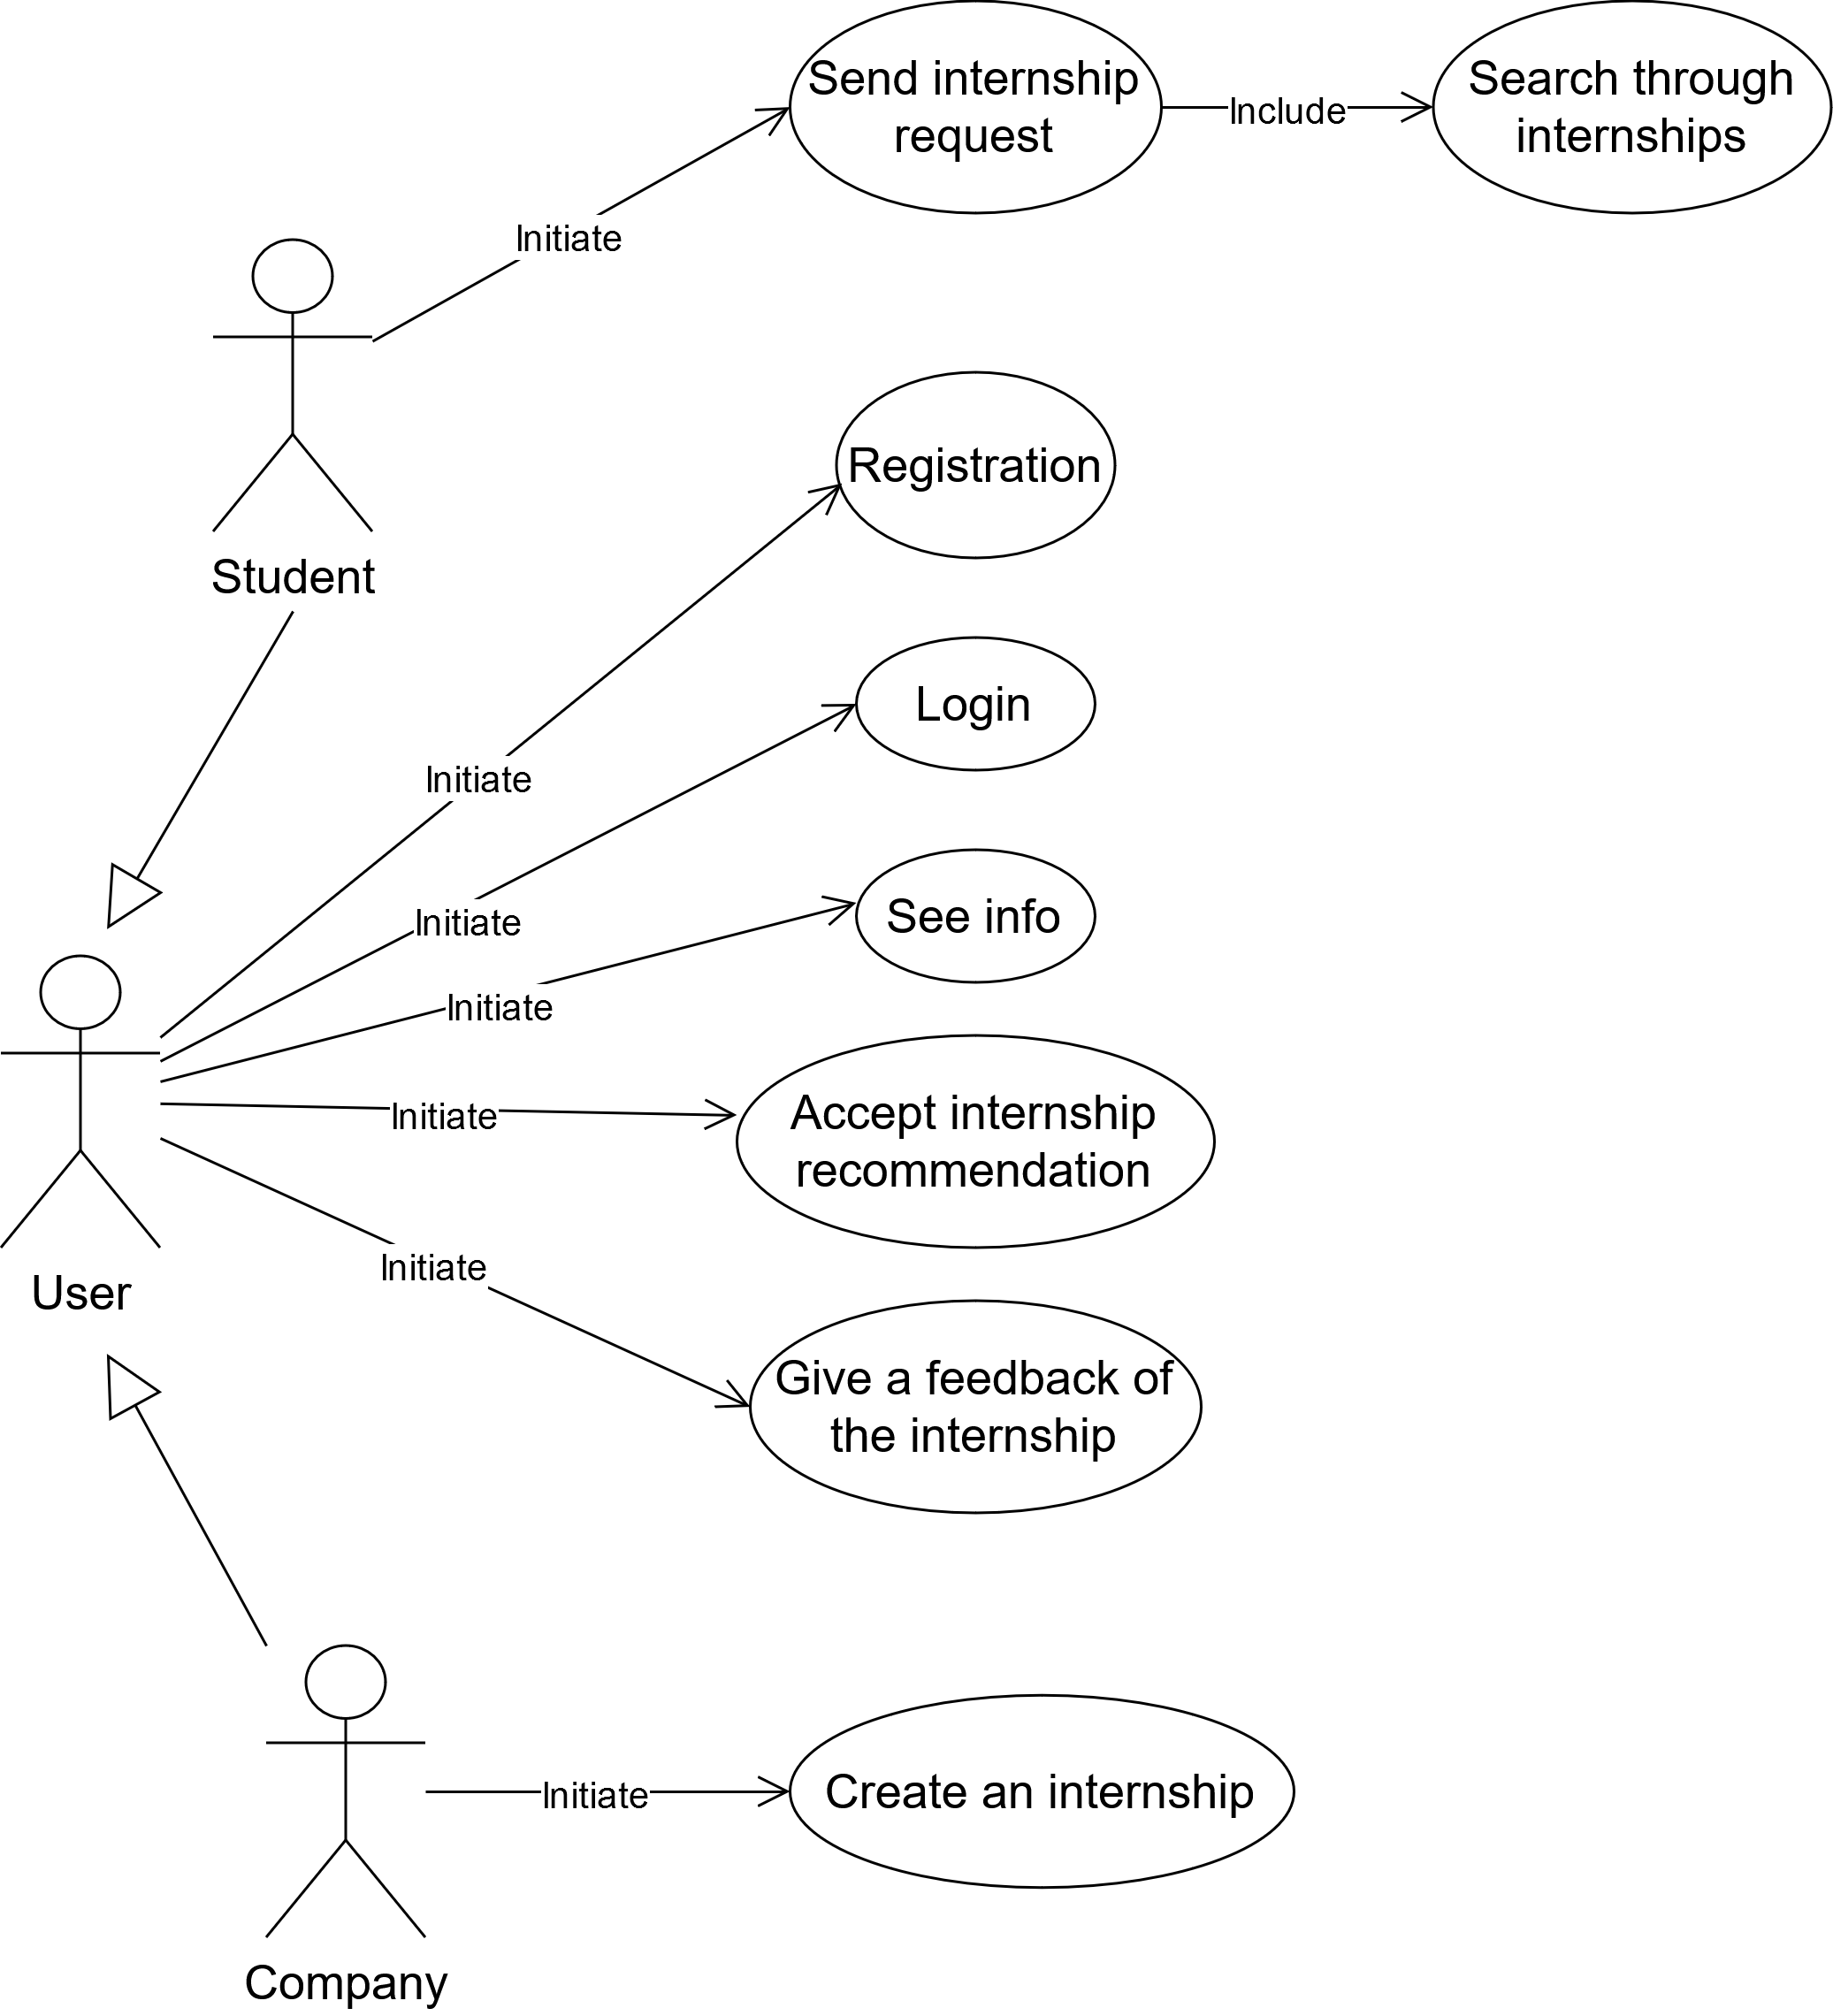
\includegraphics[width=0.75\linewidth]{Images/UseCasesDiagrams.png}
    \caption{Use Cases Diagram}
    \label{Use Cases Diagram}
\end{figure}\subsubsection{Use cases and related diagrams}

%uc1
\begin{table}[H]
\renewcommand\arraystretch{1.25}
    \centering
    \begin{tabular}{|l|p{12cm}|}
        \hline
        \textbf{Name} & Register user\\
        \hline
        \textbf{Actors} & User\\
        \hline
        \textbf{Entry conditions} & User has opened the platform\\
        \hline
        \textbf{Event flow} & 
        \begin{enumerate}
            \item The User requests to register.
            \item The system asks the user to choose if it is a Student or a Company and to provide relative data.
            \item User submits all necessary information.
            \item The system checks if email has been already used by another user to register.
            \item System updates the database with the User’s information and displays a message of confirmed registration. 
        \end{enumerate}\\
        \hline
        \textbf{Exit conditions} & User has successfully registered \\
        \hline
        \textbf{Exception} & User provides an email already registered in the database. The system displays an error.\\
        \hline
    \end{tabular}
    \caption{UC1}
    \label{UC1}
\end{table}

\begin{figure}[H]
    \centering
    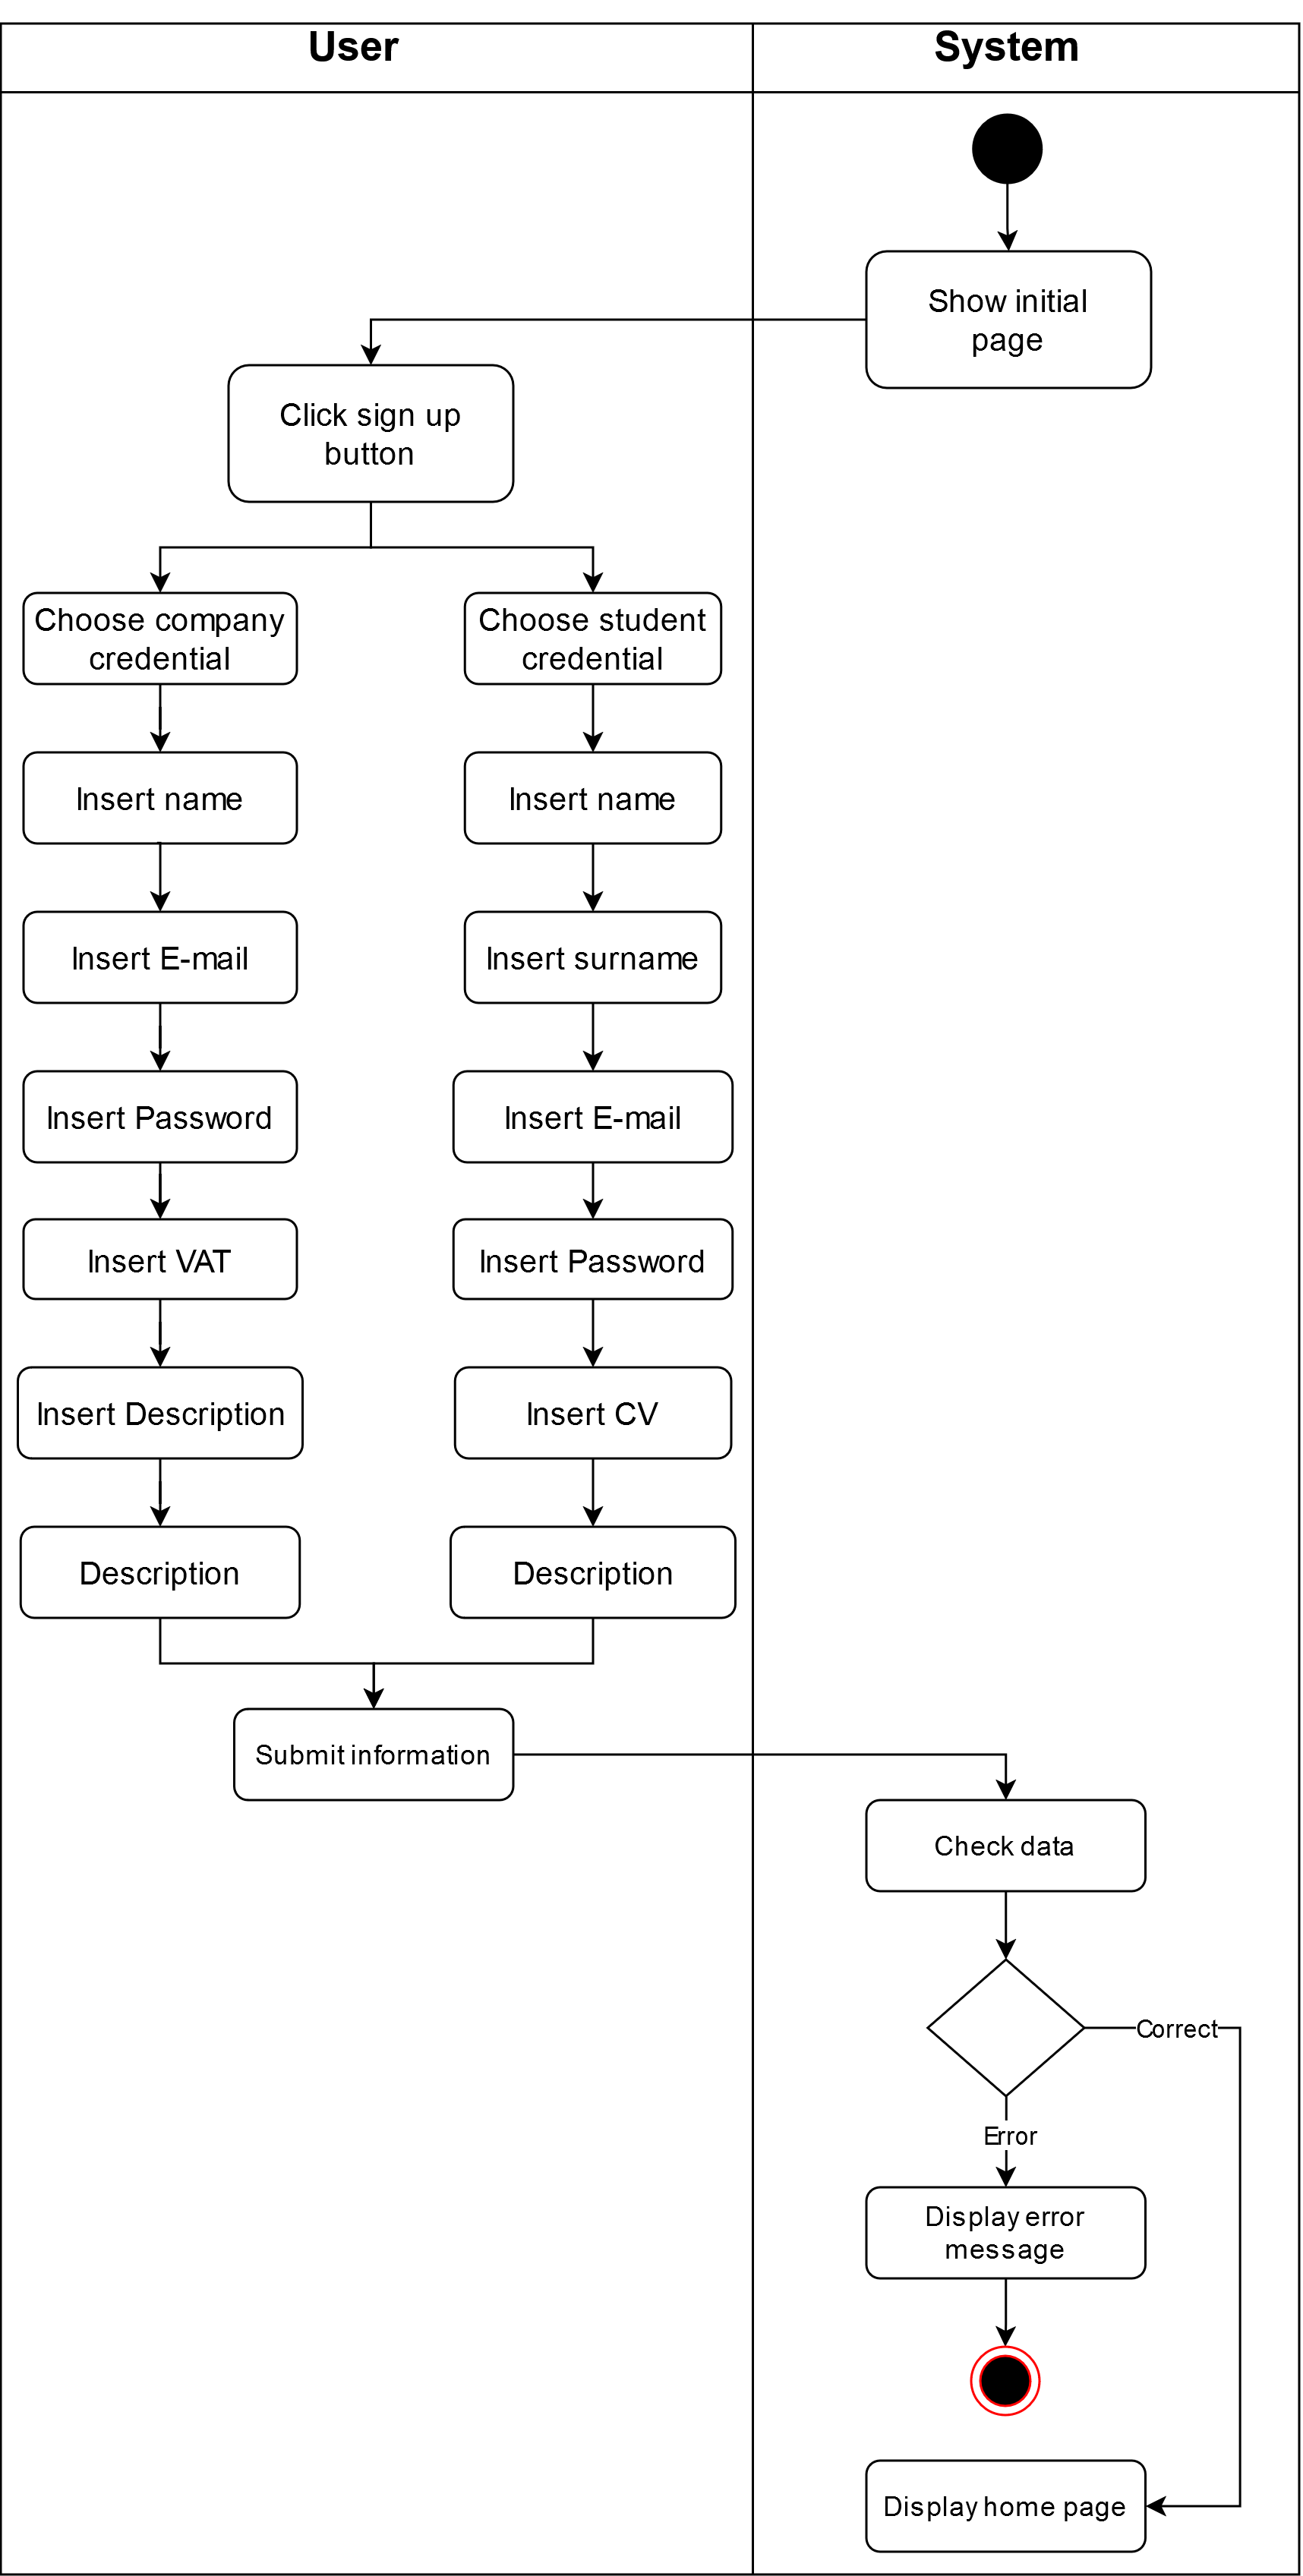
\includegraphics[width=0.75\linewidth]{Images/UseCasesDiagrams-Register.png}
    \caption{AD1}
    \label{AD1}
\end{figure}

%uc2
\begin{table}[H]
\renewcommand\arraystretch{1.25}
    \centering
    \begin{tabular}{|l|l|}
    \hline
    \textbf{Name} & Login user\\
    \hline
    \textbf{Actors} & User\\
    \hline
    \textbf{Entry conditions} & User has registered to the platform \\
    \hline
    \textbf{Events flow} &
    \begin{tabular}[c]{@{}l@{}}
    1. User inserts in apposite fields the credentials for logging in \\(username and password) and presses the “Login” button\\
    2. The system checks the correctness of the credentials inserted\\
    3. The system displays the home page\\
    \end{tabular}\\
    \hline
    \textbf{Exit conditions} & User is logged in \\
    \hline
    \textbf{Exception} & \begin{tabular}[c]{@{}l@{}}
    User inserts wrong combina
    tion of credentials and presses Login button.\\
    In this case, the application displays the Login page with an error\\
    \end{tabular}\\
    \hline
    \end{tabular}
    \caption{UC2}
    \label{UC2}
\end{table}

\begin{figure}[H]
    \centering
    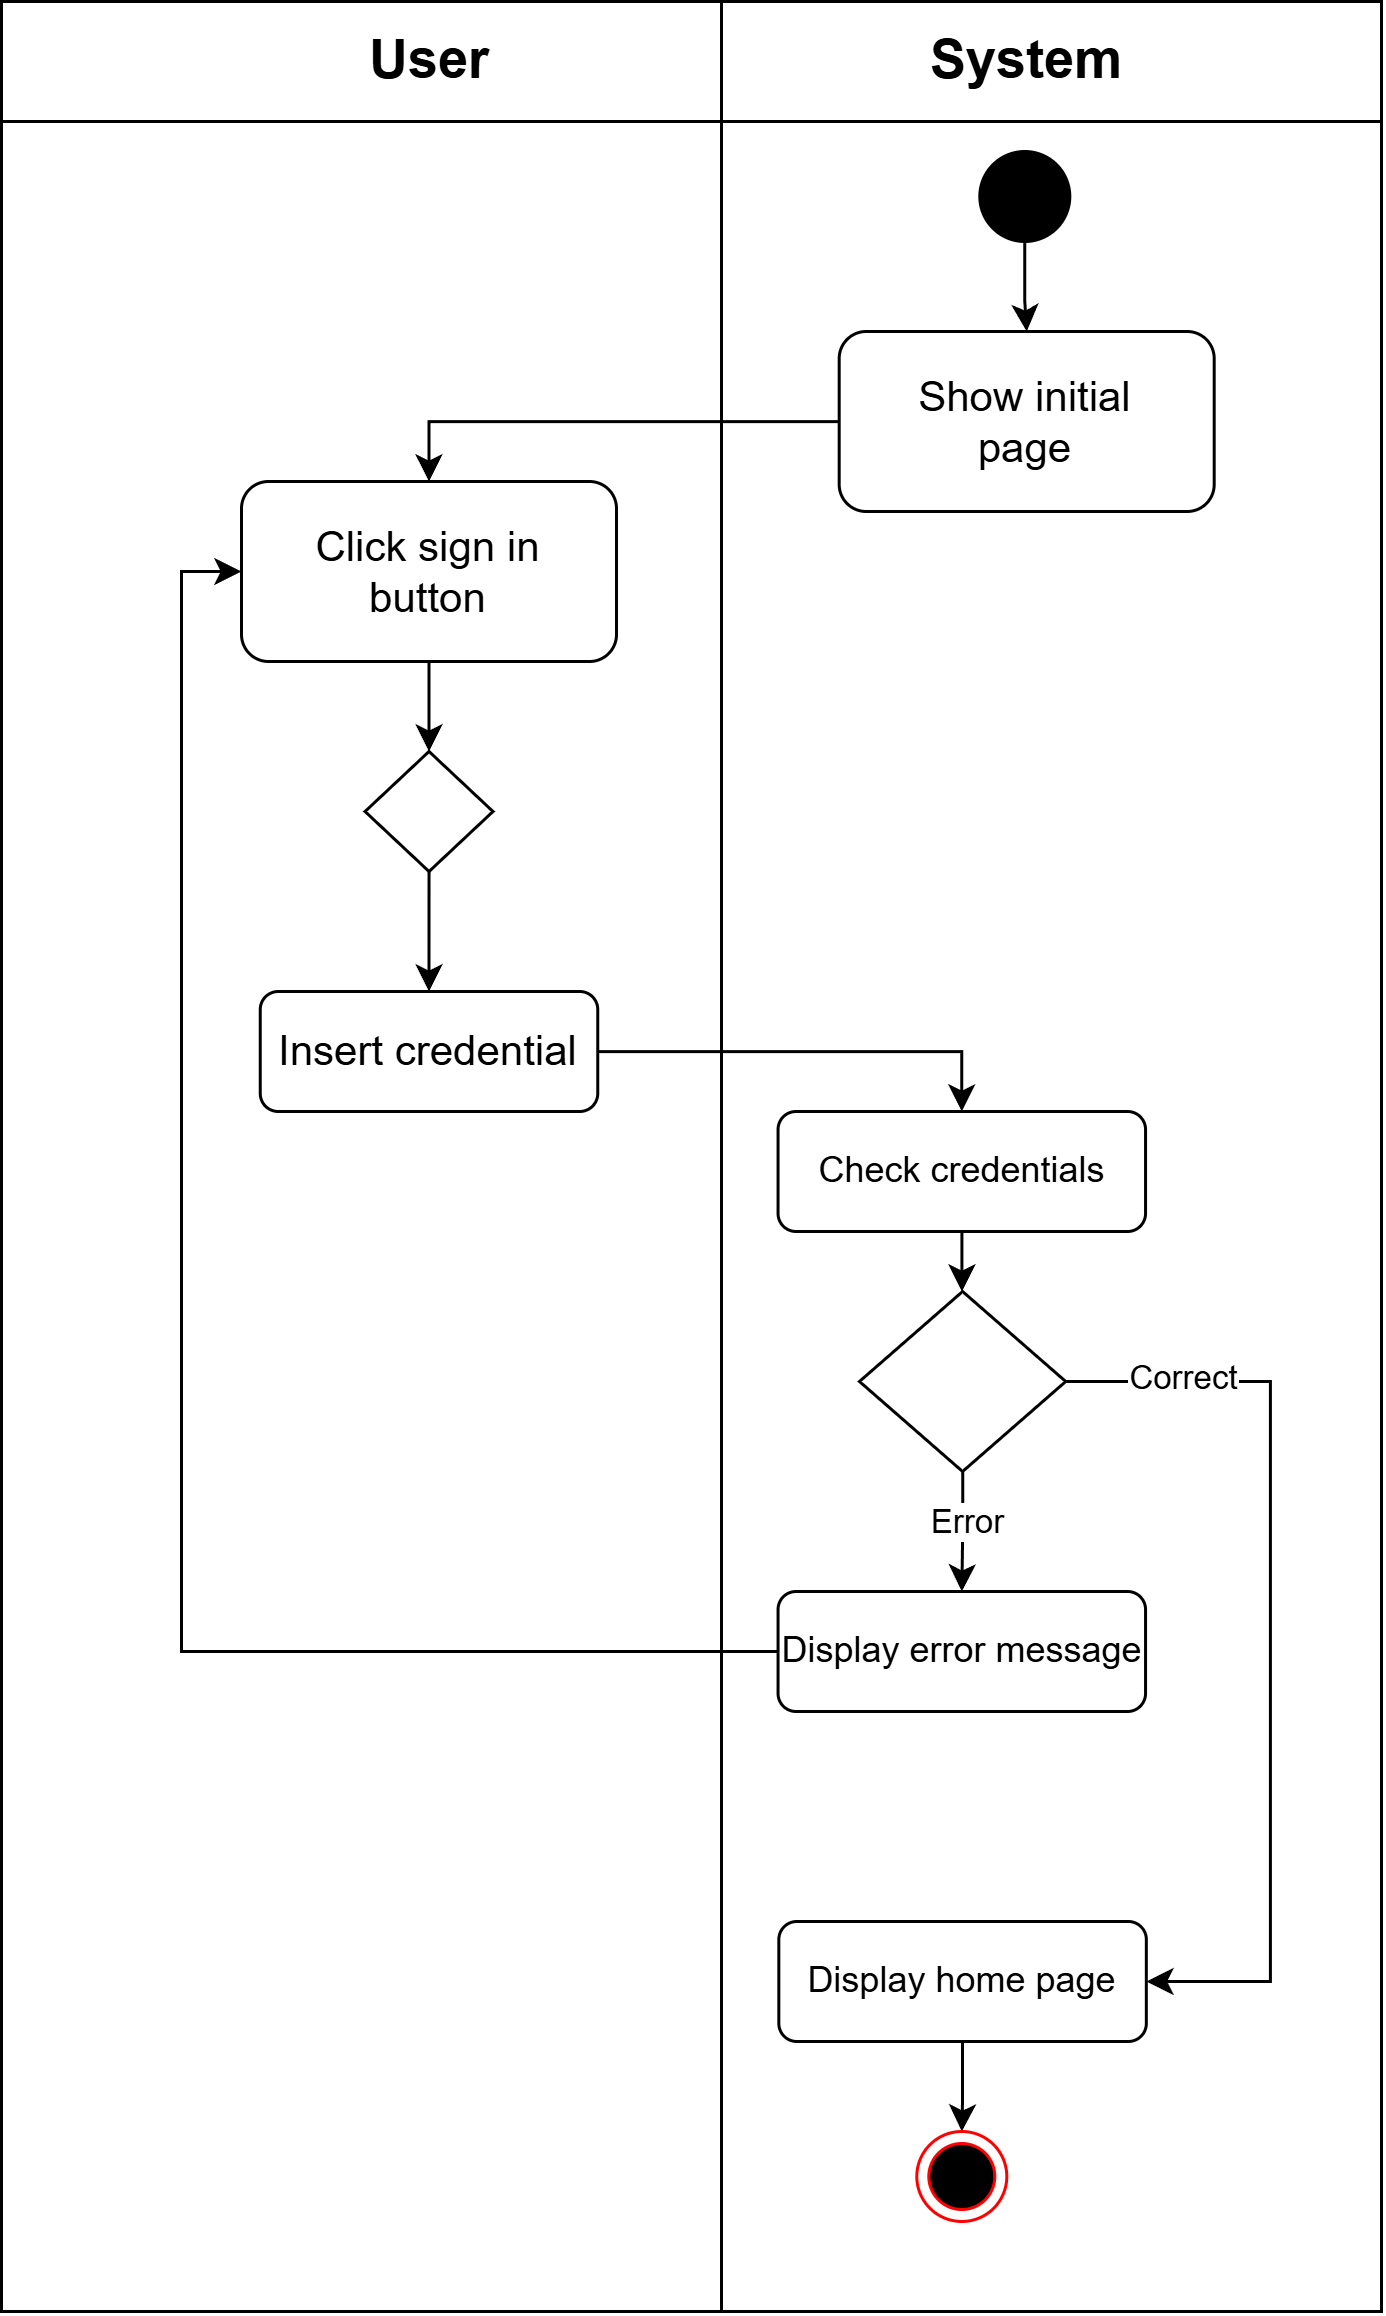
\includegraphics[width=0.75\linewidth]{Images/UseCasesDiagrams-Login.png}
    \caption{AD2}
    \label{AD2}
\end{figure}

%uc3
\begin{table}[H]
\renewcommand\arraystretch{1.25}
    \centering
    \begin{tabular}{|l|p{12 cm}|}
    \hline
    \textbf{Name} & User data management\\
    \hline
    \textbf{Actors} & User\\
    \hline
    \textbf{Entry conditions} & User has logged in to the platform \\
    \hline
    \textbf{Events flow} &
    \begin{enumerate}
        \item System show home page.
        \item User click on button "My data".
        \item System show user data.
        \item User click on button "Modify data".
        \item User can modify its information.
        \item User click on button "insert".
        \item System check validity.
        \item System shows the data updated.
    \end{enumerate}\\
    \hline
    \textbf{Exit conditions} & Company insert a valid internship \\
    \hline
    \textbf{Exception} & \begin{tabular}[c]{@{}l@{}}
    User change e-mail, inserts a not valid one and presses insert button.\\
    In this case, the application displays the Home page with an error\\
    \end{tabular}\\
    \hline
    \end{tabular}
    \caption{UC3}
    \label{UC3}
\end{table}

\begin{figure}[H]
    \centering
    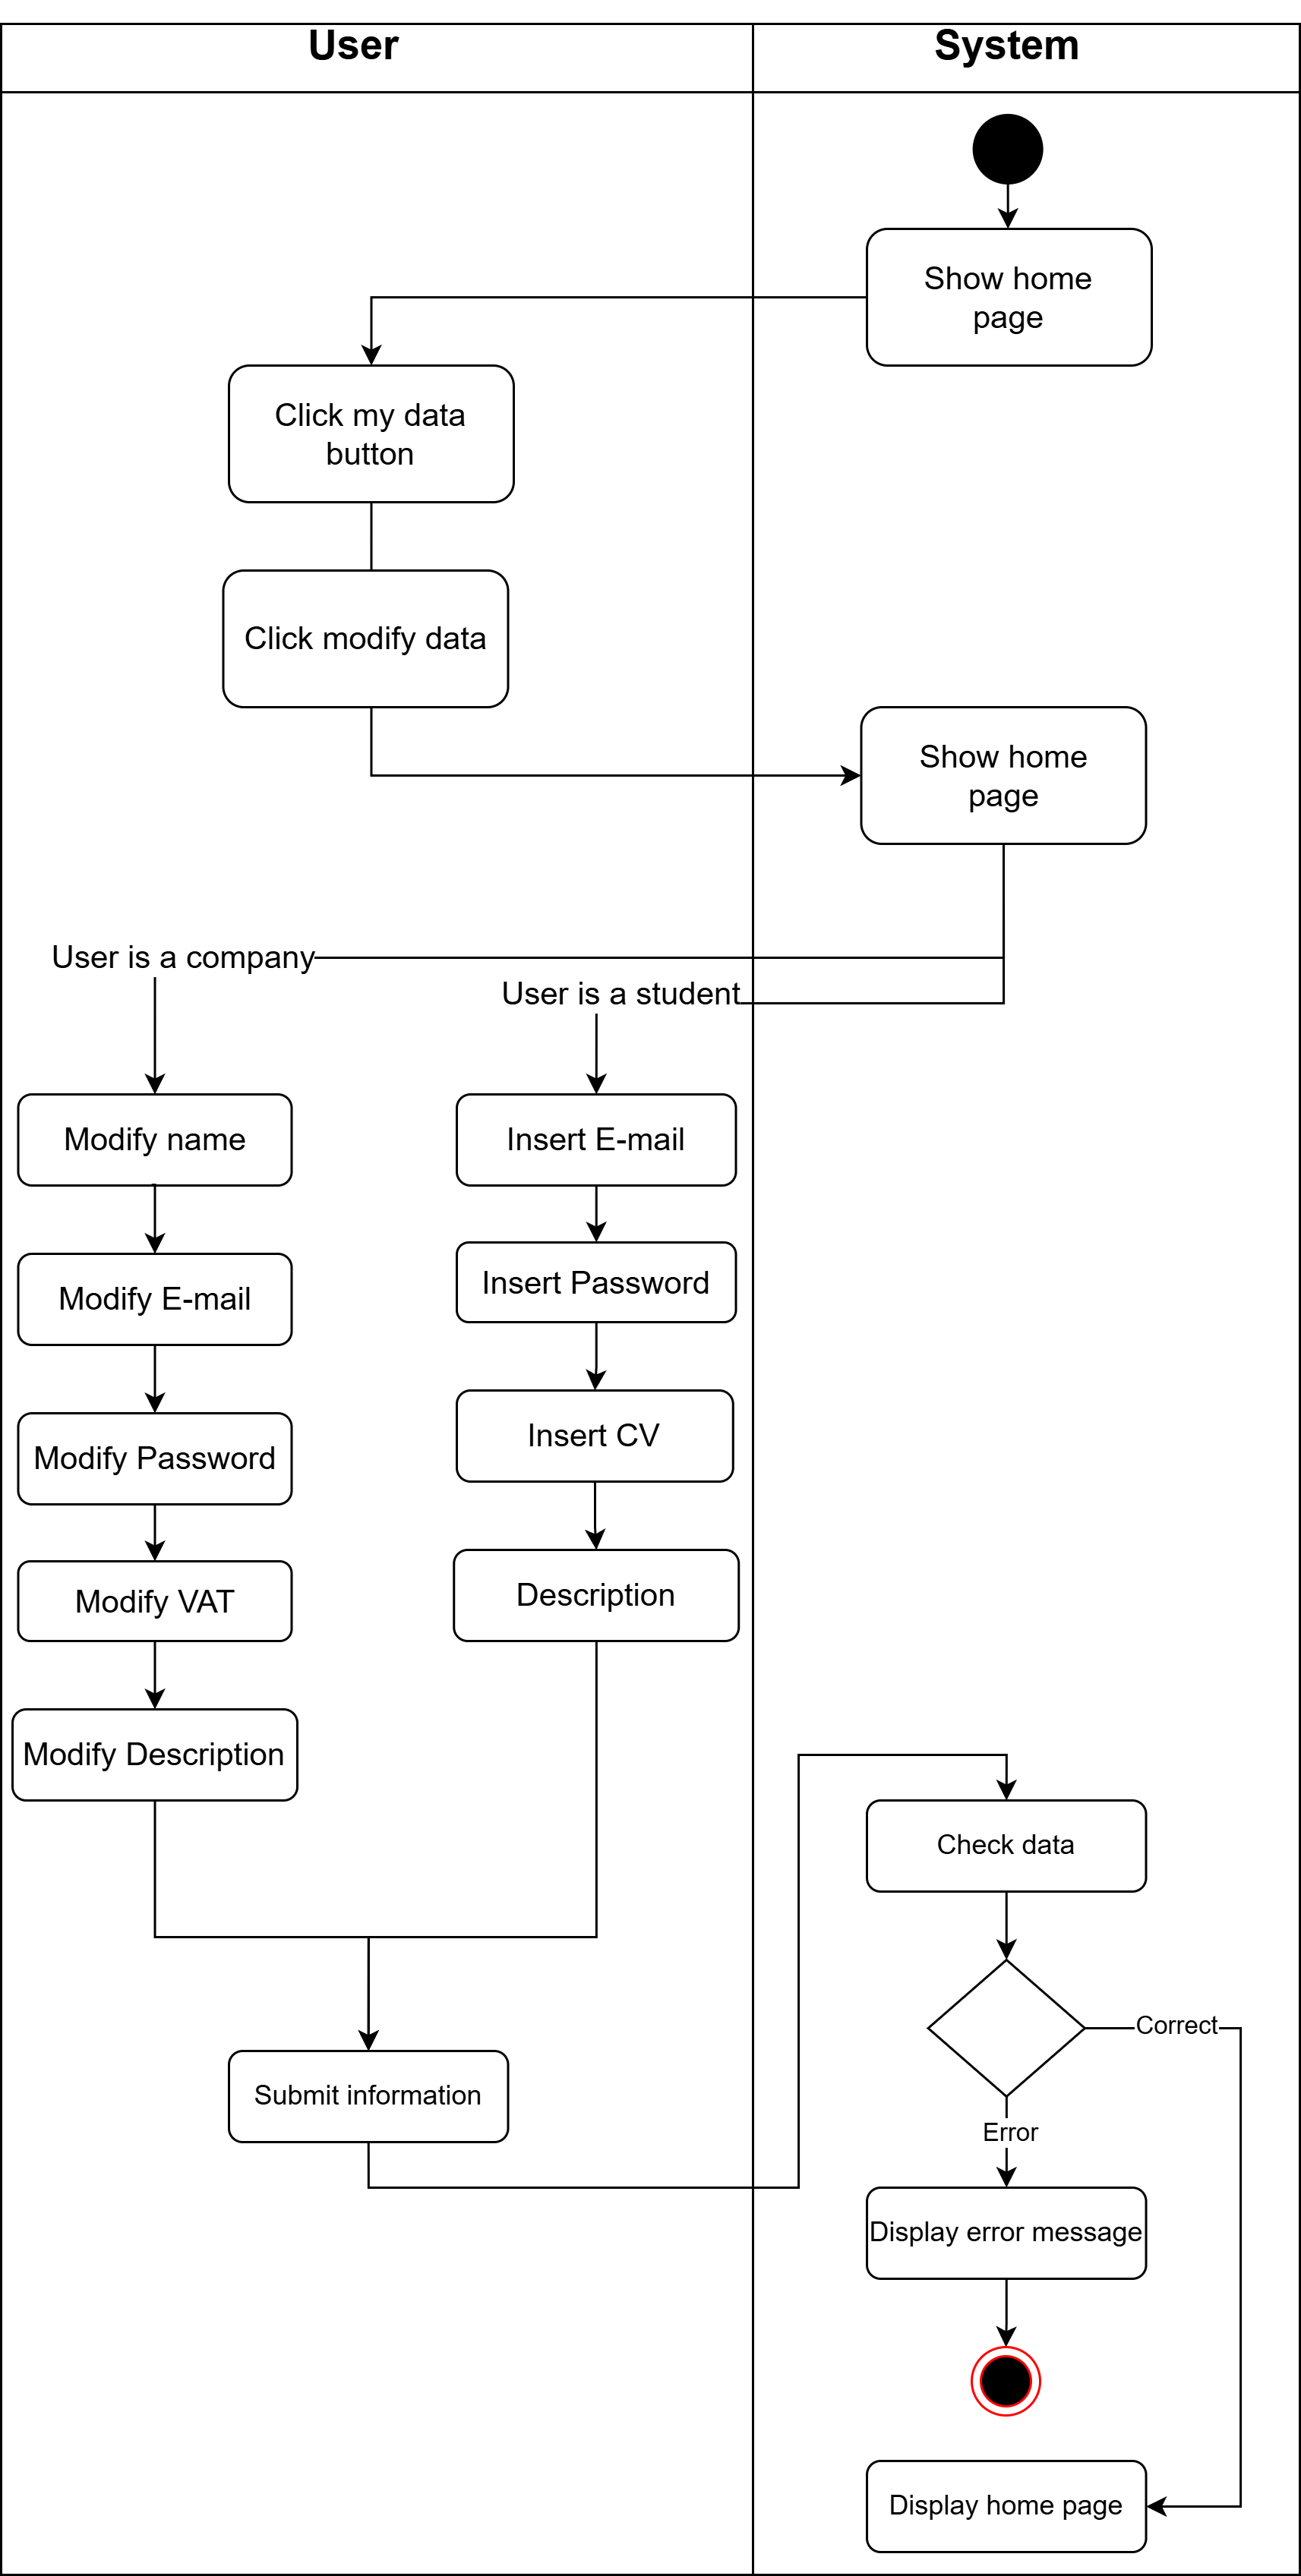
\includegraphics[width=0.7\linewidth]{Images/UseCasesDiagrams-manage-data.png}
    \caption{AD3}
    \label{AD3}
\end{figure}

%uc4
\begin{table}[H]
\renewcommand\arraystretch{1.25}
    \centering
    \begin{tabular}{|l|p{12 cm}|}
    \hline
    \textbf{Name} & Internship insertion\\
    \hline
    \textbf{Actors} & Company\\
    \hline
    \textbf{Entry conditions} & Company has registered/logged in to the platform \\
    \hline
    \textbf{Events flow} &
    \begin{enumerate}
        \item System show the home page.
        \item Company click on button insert "new internship".
        \item Company insert valid information of an "internship", such as name, start date, end date, salary, qualification required and a description.
        \item Company click on button "insert".
        \item System check validity.
        \item System shows the inserted internship list updated.
    \end{enumerate}\\
    \hline
    \textbf{Exit conditions} & Company insert a valid internship \\
    \hline
    \textbf{Exception} & \begin{tabular}[c]{@{}l@{}}
    Company inserts a not valid date and presses insert button.\\
    In this case, the application displays the Home page with an error\\
    \end{tabular}\\
    \hline
    \end{tabular}
    \caption{UC4}
    \label{UC4}
\end{table}

\begin{figure}[H]
    \centering
    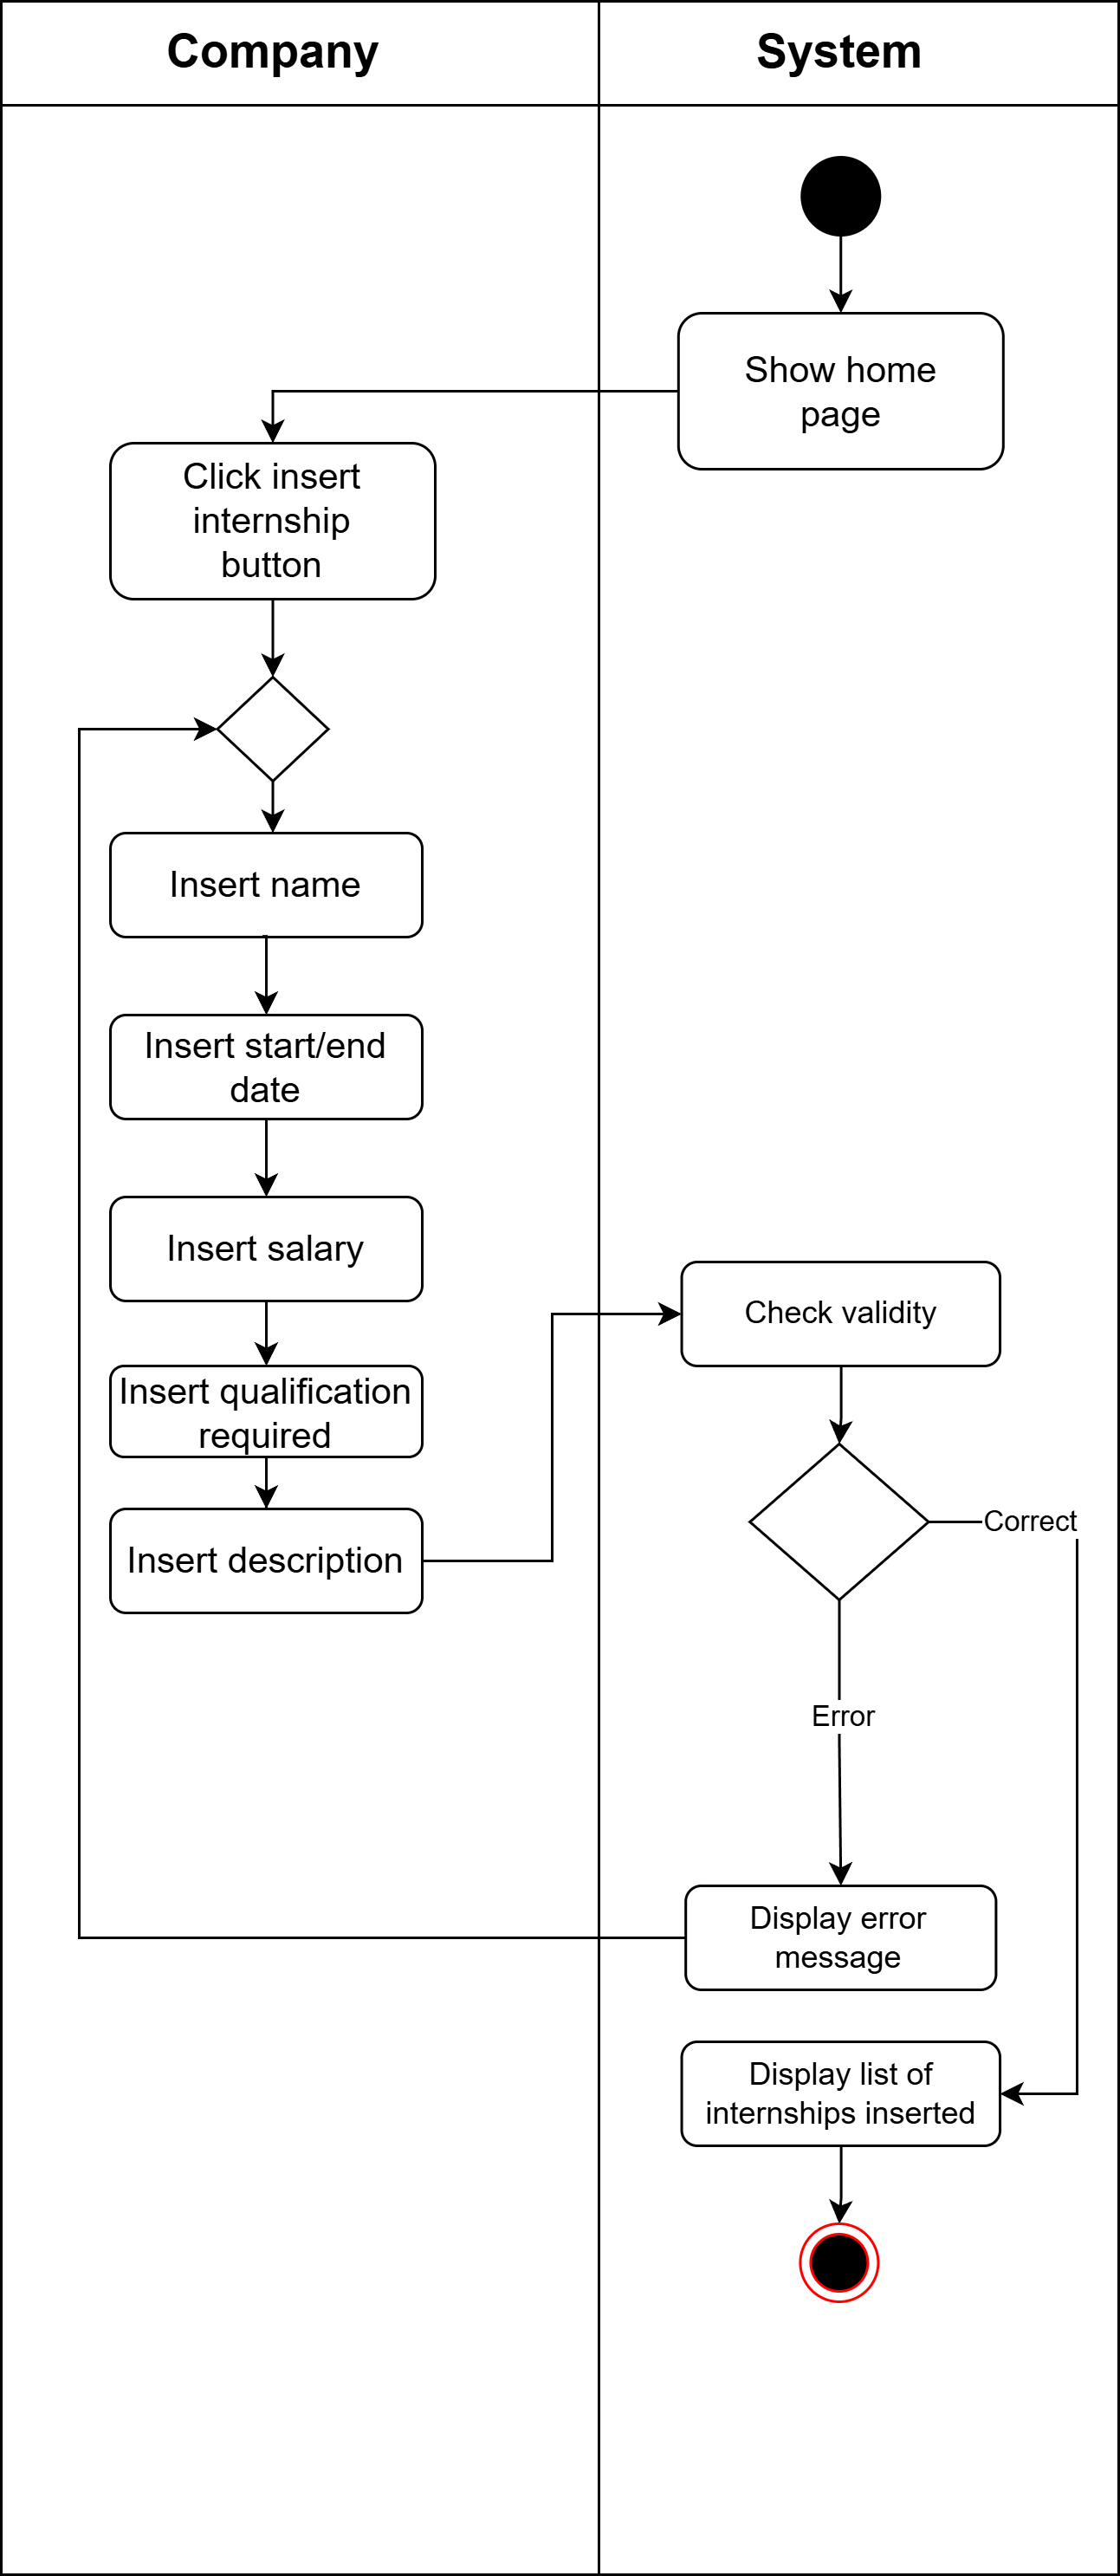
\includegraphics[width=0.65\linewidth]{Images/insert_internship.png}
    \caption{AD4}
    \label{AD4}
\end{figure}

%uc5
\begin{table}[H]
\renewcommand\arraystretch{1.25}
    \centering
    \begin{tabular}{|l|p{12 cm}|}
    \hline
    \textbf{Name} & Internship modification\\
    \hline
    \textbf{Actors} & Company\\
    \hline
    \textbf{Entry conditions} & Company has logged in to the platform \\
    \hline
    \textbf{Events flow} &
    \begin{enumerate}
        \item System shows home page.
        \item Company click on button "My internship".
        \item Company click on button "Modify internship".
        \item Company can modify information of an "internship", such as name, start date, end date, salary, qualification required and a description.
        \item Company click on button "insert".
        \item System check validity.
        \item System shows the inserted internship list updated.
    \end{enumerate}\\
    \hline
    \textbf{Exit conditions} & Company insert a valid internship \\
    \hline
    \textbf{Exception} & \begin{tabular}[c]{@{}l@{}}
    Company inserts a not valid date and presses insert button.\\
    In this case, the application displays the Home page with an error\\
    \end{tabular}\\
    \hline
    \end{tabular}
    \caption{UC5}
    \label{UC5}
\end{table}

\begin{figure}[H]
    \centering
    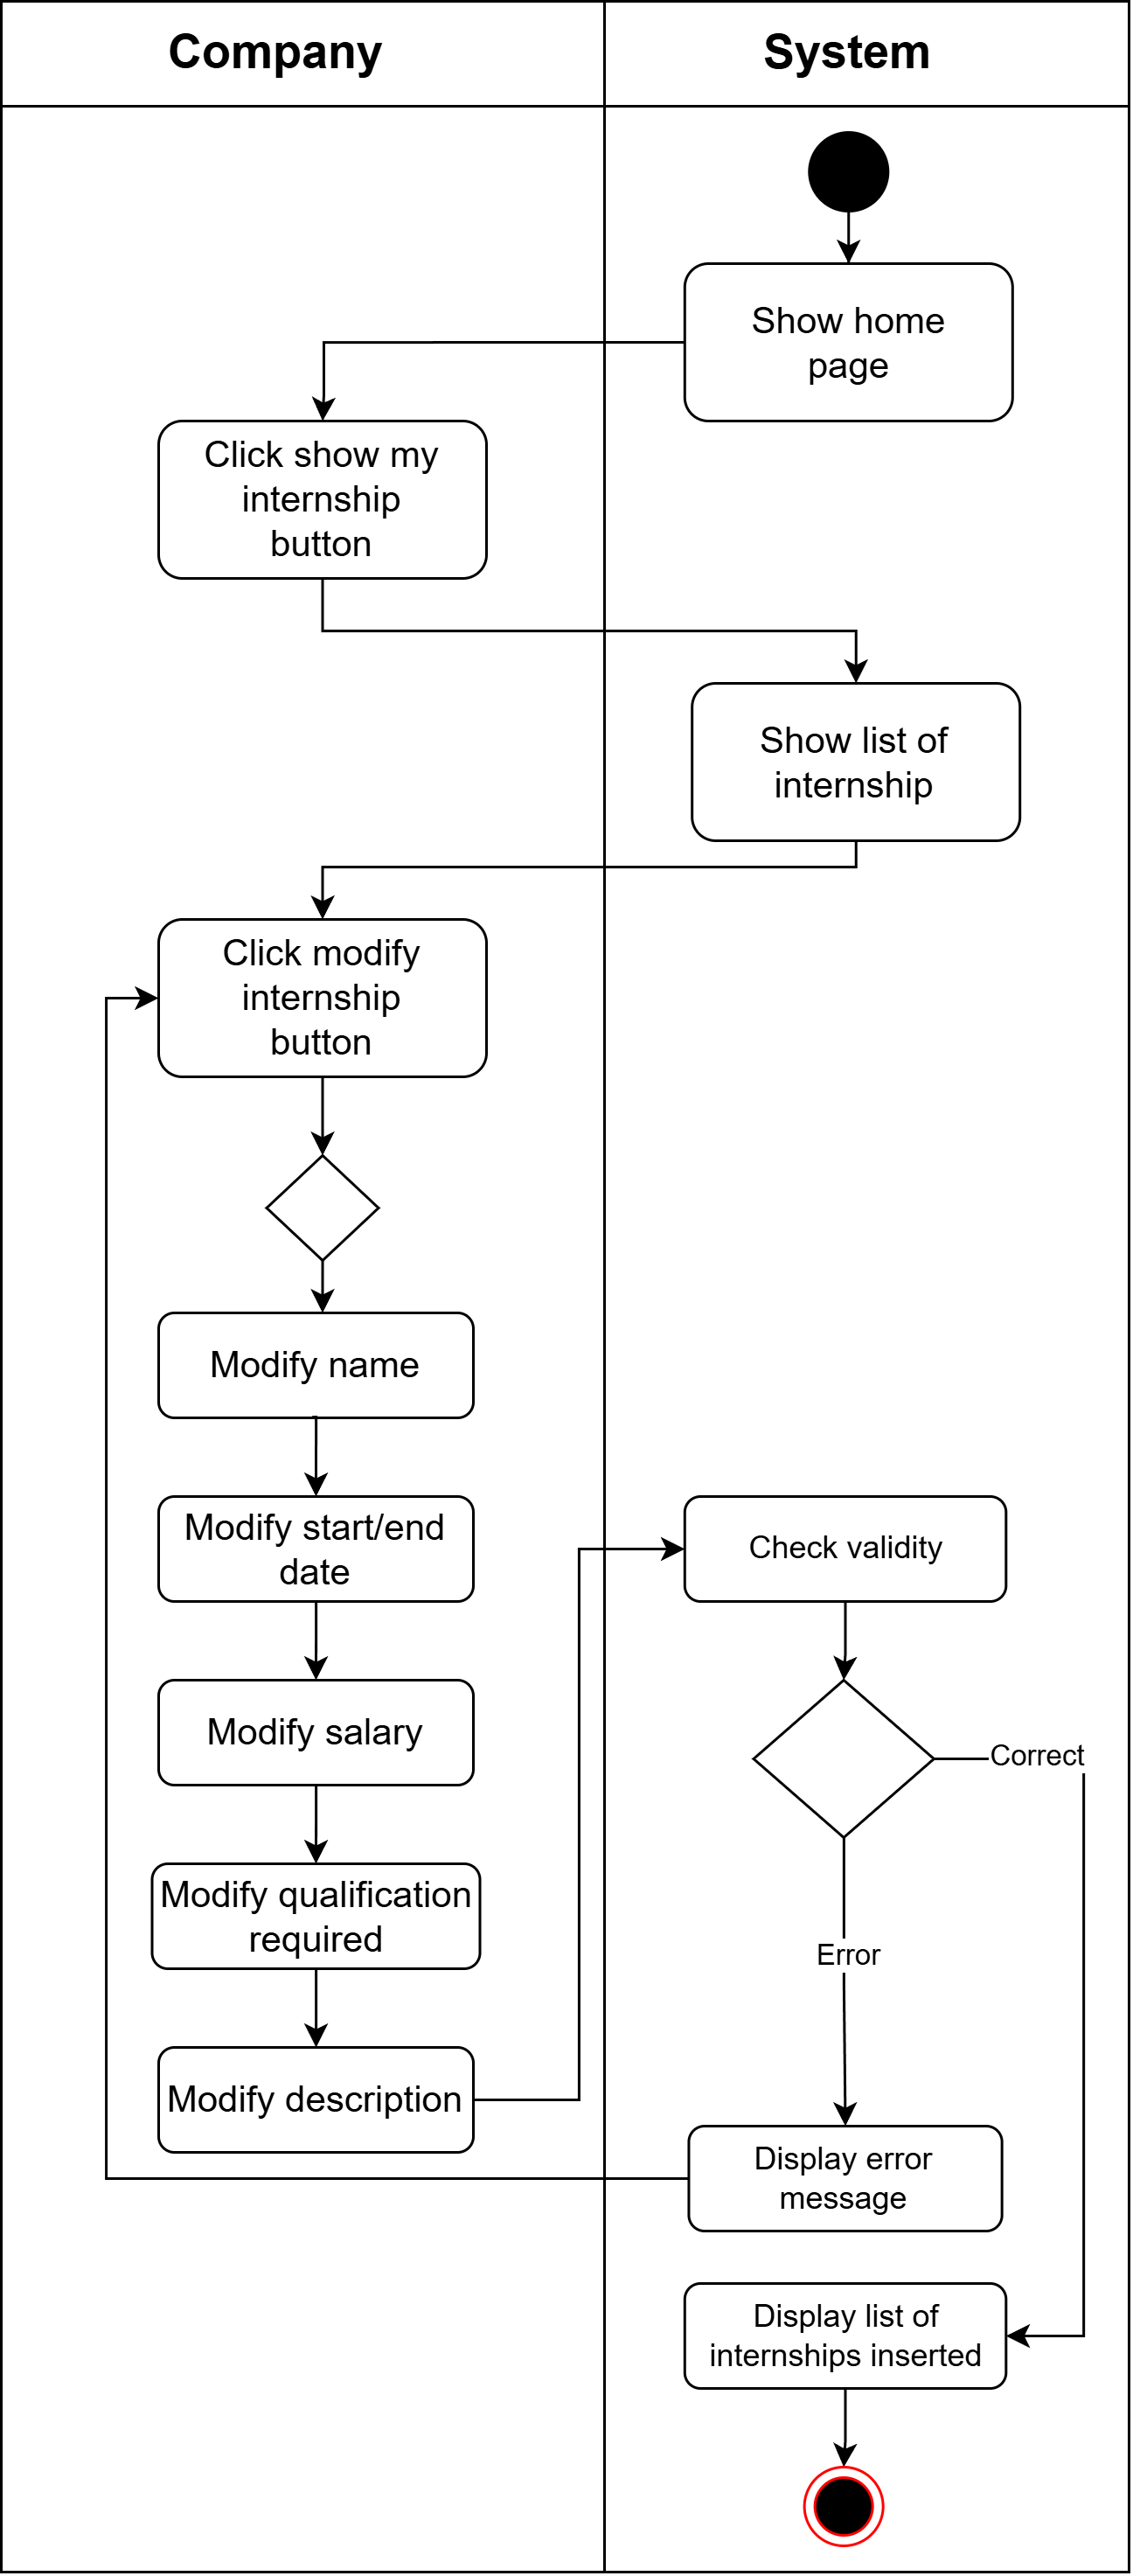
\includegraphics[width=0.6\linewidth]{Images/UseCasesDiagrams-UC modify-internship.png}
    \caption{AD5}
    \label{AD5}
\end{figure}

%uc6
\begin{table}[H]
\renewcommand\arraystretch{1.25}
    \centering
    \begin{tabular}{|l|p{12 cm}|}
    \hline
    \textbf{Name} & Student proactive search\\
    \hline
    \textbf{Actors} & Student\\
    \hline
    \textbf{Entry conditions} & Student has logged in to the platform\\
    \hline
    \textbf{Events flow} &
    \begin{enumerate}
        \item System shows the list of available internship in home page and a search bar.
        \item Student search through the list.
        \begin{enumerate}
            \item Student scroll and click button "show details".
            \item Student write a keyword on the search bar and press the button "search".
            \begin{enumerate}
                \item System produce some results
                \item Student scroll the list of result and click button "show details".
            \end{enumerate}
        \end{enumerate}
        \item System shows the selected internship information.
    \end{enumerate}\\  
    \hline
    \textbf{Exit conditions} & 
    \begin{enumerate}[label=(\alph*)]
        \item Student click on button "Ask for an internship".
        \item Student click on button "Close the research"
    \end{enumerate}\\
    \hline
    \textbf{Exception} & Search does not produce results, the application produce an error message and goes back to the full list\\
    \hline
    \end{tabular}
    \caption{UC6}
    \label{UC6}
\end{table}

\begin{figure}[H]
    \centering
    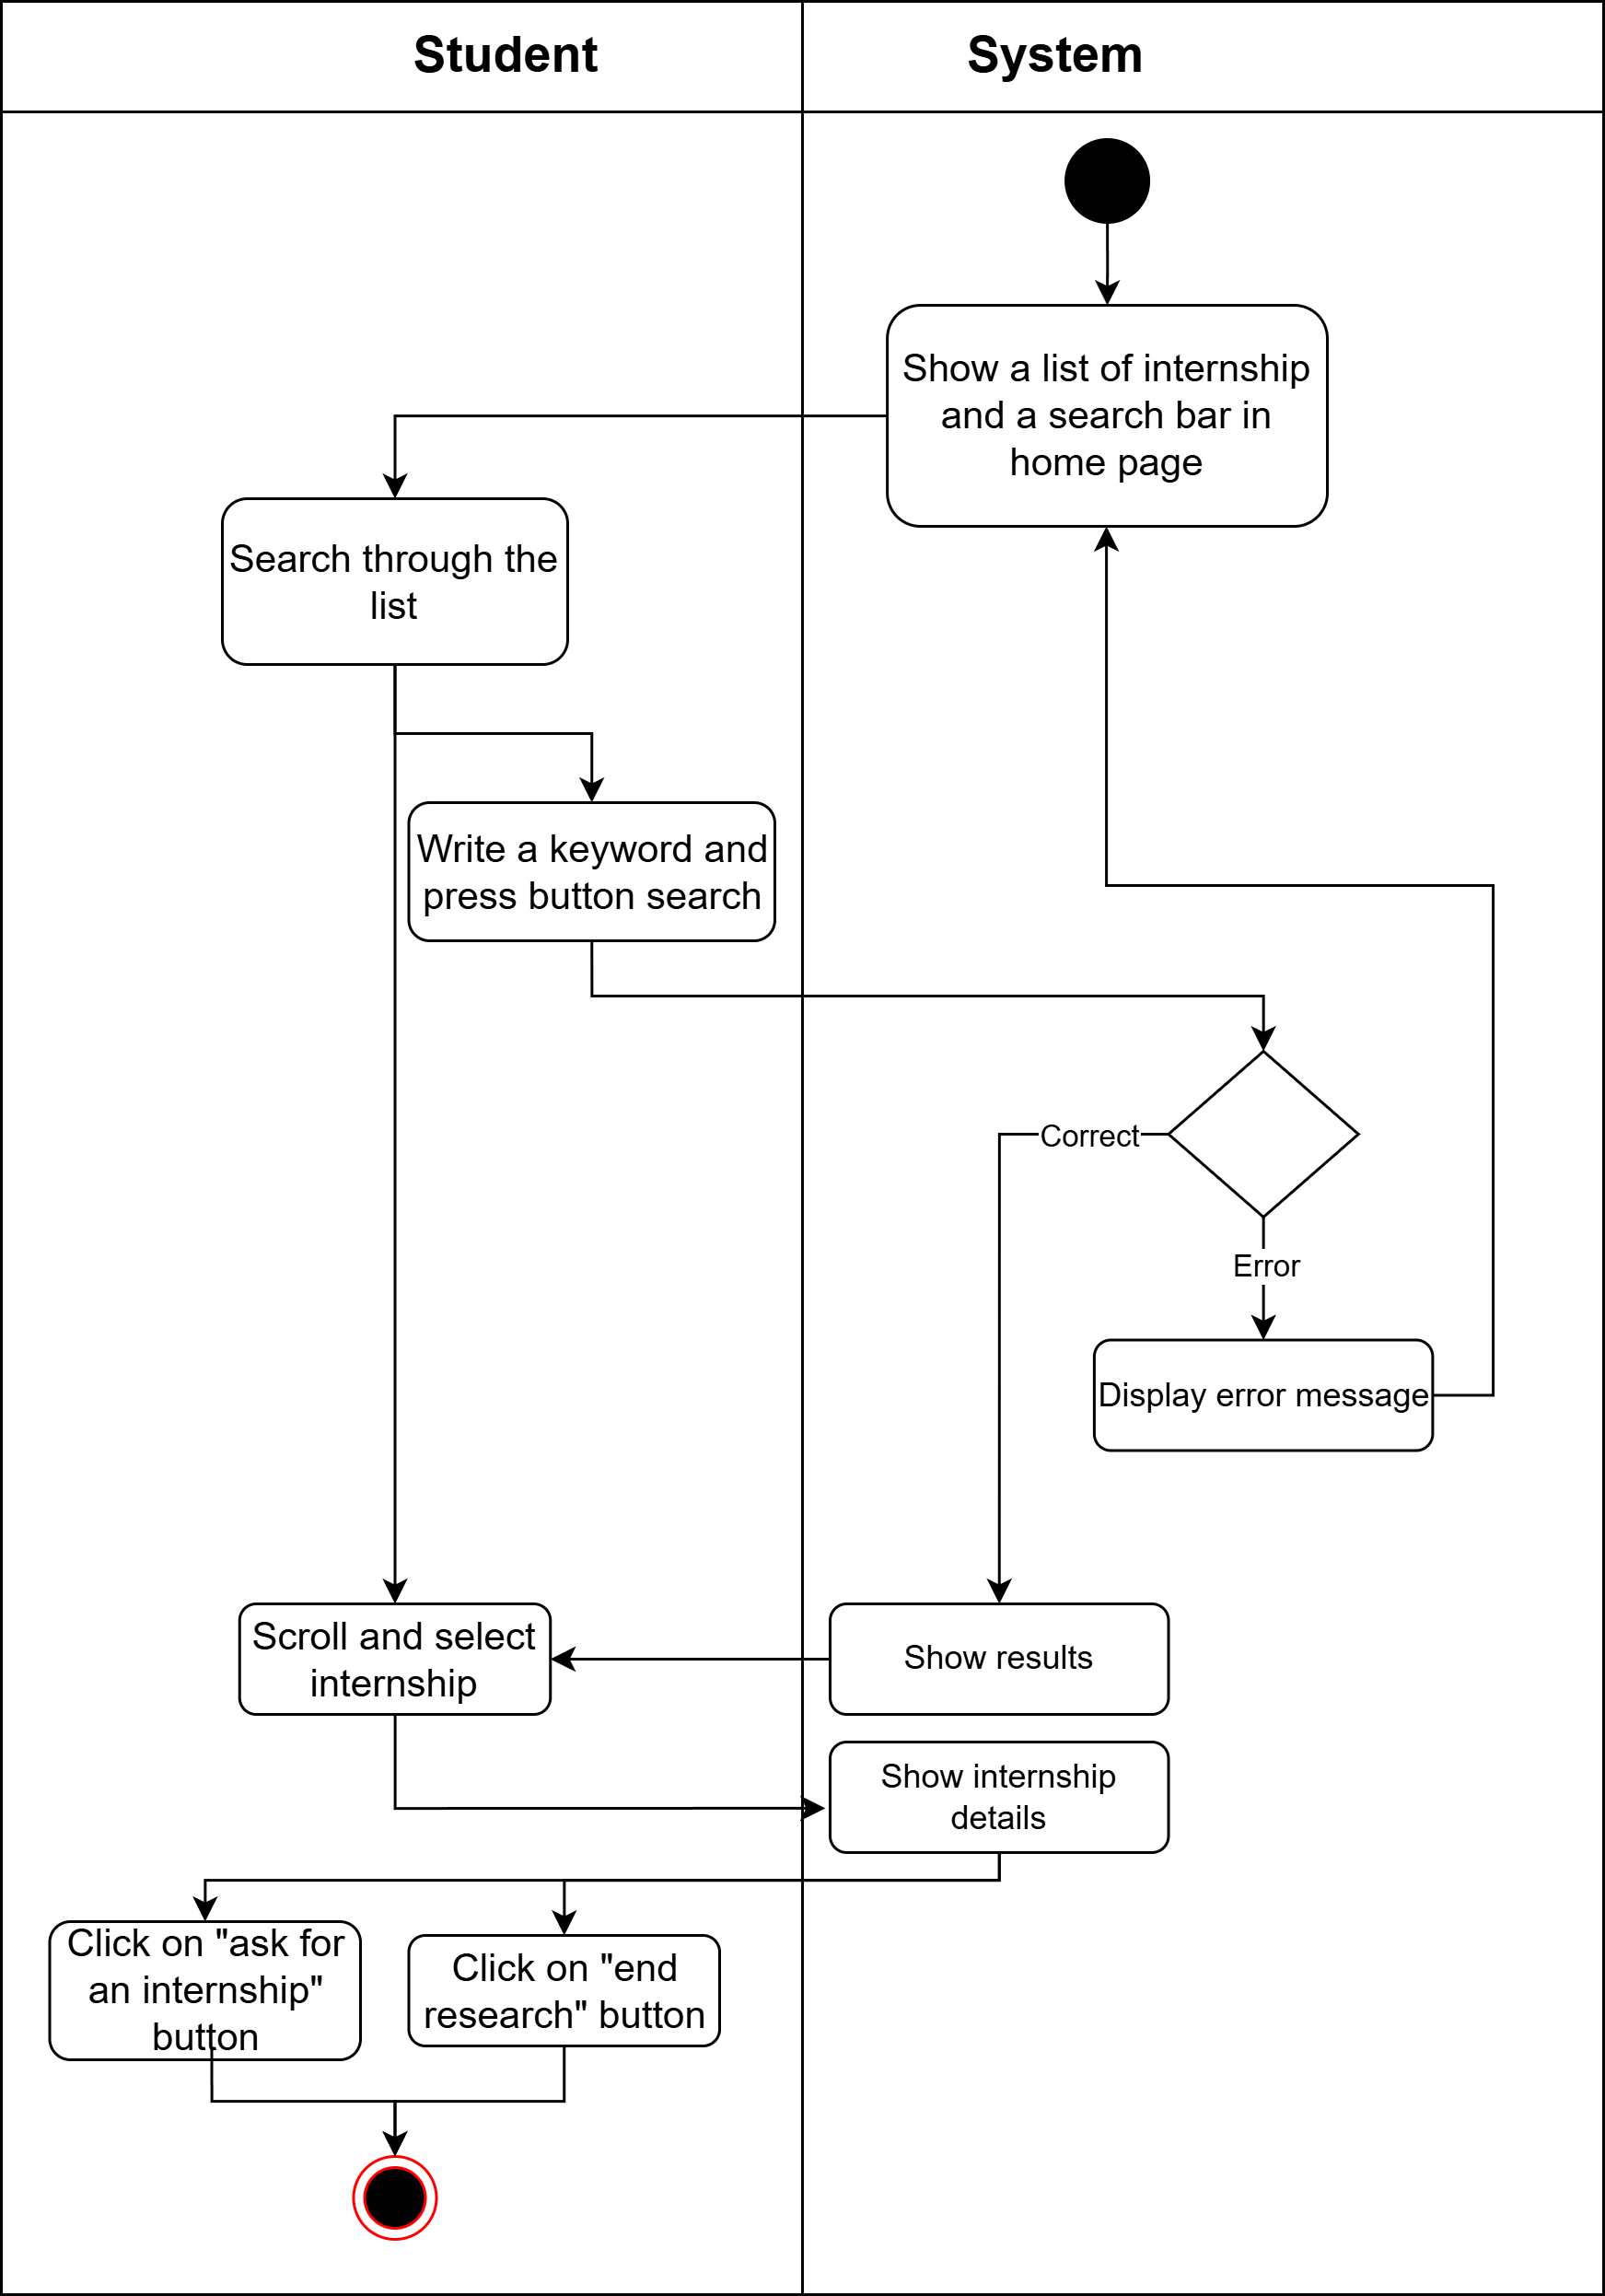
\includegraphics[width=1\linewidth]{Images/UseCasesDiagrams-Student search.png}
    \caption{AD6}
    \label{AD6}
\end{figure}

%uc7
\begin{table}[H]
\renewcommand\arraystretch{1.25}
    \centering
    \begin{tabular}{|l|p{12 cm}|}
    \hline
    \textbf{Name} & Student notification\\
    \hline
    \textbf{Actors} & Student\\
    \hline
    \textbf{Entry conditions} & Recommendation system find a match.\\
    \hline
    \textbf{Events flow} & The notification appears on the main page of the student.\\  
    \hline
    \textbf{Exit conditions} & 
    \begin{enumerate}[label=(\alph*)]
        \item The student decides to accept the internship.
        \item The student decides to reject the internship.
    \end{enumerate}\\
    \hline
    \end{tabular}
    \caption{UC7}
    \label{UC7}
\end{table}

%uc8
\begin{table}[H]
\renewcommand\arraystretch{1.25}
    \centering
    \begin{tabular}{|l|p{12 cm}|}
    \hline
    \textbf{Name} & Company notification\\
    \hline
    \textbf{Actors} & Company\\
    \hline
    \textbf{Entry conditions} & 
    \begin{enumerate}[label=(\alph*)]
        \item A student click the button "Ask for an internship".
        \item Recommendation system find a match.
    \end{enumerate}\\
    \hline
    \textbf{Events flow} & The notification appears on the main page of the company.\\  
    \hline
    \textbf{Exit conditions} & 
    \begin{enumerate}[label=(\alph*)]
        \item The company decides to accept the internship.
        \item The company decides to reject the internship.
    \end{enumerate}\\
    \hline
    \end{tabular}
    \caption{UC8}
    \label{UC8}
\end{table}

%uc9
\begin{table}[H]
\renewcommand\arraystretch{1.25}
    \centering
    \begin{tabular}{|l|p{12 cm}|}
    \hline
    \textbf{Name} & User schedule the interview\\
    \hline
    \textbf{Actors} & Student and company\\
    \hline
    \textbf{Entry conditions} & 
    \begin{enumerate}[label=(\alph*)]
        \item Company accepts the request of the student.
        \item Student and company accept the notification of the recommendation system.
    \end{enumerate}\\
    \hline
    \textbf{Events flow} &
    \begin{enumerate}
        \item User clicks on accepted internship.
        \item User clicks on the calendar icon.
        \item The system shows the calendar.
        \item User the user indicates which days he has free.
    \end{enumerate}\\  
    \hline
    \textbf{Exit conditions} & 
    \begin{enumerate}[label=(\alph*)]
        \item User click the button "save".
        \item User click out the calendar.
    \end{enumerate}\\
    \hline
    \textbf{Exception} & User click the button "save" without indicate the free days\\
    \hline
    \end{tabular}
    \caption{UC9}
    \label{UC9}
\end{table}

%uc11
\begin{table}[H]
\renewcommand\arraystretch{1.25}
    \centering
    \begin{tabular}{|l|p{12 cm}|}
    \hline
    \textbf{Name} & User leave a feedback\\
    \hline
    \textbf{Actors} & Student and company\\
    \hline
    \textbf{Entry conditions} & The internship is over\\
    \hline
    \textbf{Events flow} &
    \begin{enumerate}
        \item User clicks on  finished internship.
        \item The system shows a box where you can write it.
        \item User write the feedback.
    \end{enumerate}\\  
    \hline
    \textbf{Exit conditions} & User click the button "save"\\
    \hline
    \end{tabular}
    \caption{UC11}
    \label{UC11}
\end{table}

%uc12
\begin{table}[H]
\renewcommand\arraystretch{1.25}
    \centering
    \begin{tabular}{|l|p{12 cm}|}
    \hline
    \textbf{Name} & Zoom call \\
    \hline
    \textbf{Actors} & Student and company\\
    \hline
    \textbf{Entry conditions} & S\&C finds a free slot for both of them\\
    \hline
    \textbf{Events flow} &
    \begin{enumerate}
        \item The system communicates with Zoom to create a link for the video-call.
        \item Zoom successfully creates the link.
        \item Zoom sends the link to the system that saves it in the database.
        \item The system show the link on the users page.
    \end{enumerate}\\  
    \hline
    \textbf{Exit conditions} & On the day the internship starts the link is deleted\\
    \hline
    \end{tabular}
    \caption{UC12}
    \label{UC12}
\end{table}

\subsubsection{Requirements}

\begin{table}[H]
\renewcommand\arraystretch{1.5}
    \centering
    \begin{tabular}{ll}
    \hline
    \textbf{R1} & The S\&C platform allows users to register.\\
    \hline
    \textbf{R2} & The S\&C platform allows users to register filling mandatory fields.\\
    \hline
    \textbf{R3} & The S\&C platform allows users to login using their credential.\\
    \hline
    \textbf{R4} & The S\&C platform allows users to manage their data and modify them.\\
    \hline
    \textbf{R5} & The S\&C platform allows companies to insert an internship.\\
    \hline
    \textbf{R6} & The S\&C platform allows company to modify their internships data.\\
    \hline
    \textbf{R7} & The S\&C platform should provide the "search internship" functionality to students.\\
    \hline
    \textbf{R8} & The S\&C platform should notify users when a match is found.\\
    \hline
    \textbf{R9} & The S\&C platform should notify companies when a match is found.\\
    \hline
    \textbf{R10} & The S\&C platform should notify companies when a student request to be contacted.\\
    \hline
    \textbf{R11} & The S\&C platform should allows users to accept or not the match made by the platform.\\
    \hline
    \textbf{R12} & The S\&C platform should send to the students a form related to the chosen internship\\
    \hline
    \textbf{R13} & The user should fill the mandatory form by the deadline\\
    \hline
    \textbf{R14} & The S\&C platform check that the form has been compiled by the deadline\\
    \hline
    \textbf{R15} & The S\&C platform allows user to insert their free slots\\
    \hline
    \textbf{R16} & The S\&C platform should provide a match for a free slot between the users schedules\\
    \hline
    \textbf{R17} & \begin{tabular}[c]{@{}l@{}}The S\&C platform should be able to request zoom to create a call room\\ and receive back the corresponding link.\end{tabular}\\
    \hline
    \textbf{R18} & The S\&C platform should allows users to leave feedback. 
    \end{tabular}
    \caption{Requirements}
    \label{Requirements}
\end{table}

\subsubsection{Mapping on requirements}

\begin{table}[H]
\renewcommand\arraystretch{1.5}
    \centering
    \begin{tabular}{p{10cm}ll}
    \rowcolor{BurntOrange}
        \textbf{Goal}&  \textbf{Requirements}& \textbf{Assumptions}\\
    \hline
    \textbf{[G1]:}All unregistered students and Companies must be able to subscribe and login to the S\&C platform. & R1,R2,R3 & A1,A2,A4,A6\\
    \hline
    \textbf{[G2]:} Companies must be able to create internship offers.& R5, R6 & \\
    \hline
    \textbf{[G3]:} Students must be able to complete their CV and preferences.& R4 & \\
    \hline
    \textbf{[G4]:} Students must be able to search for an internship.& R7 & \\
    \hline
    \textbf{[G5]:} Student and Company are informed when there is a match between them.
    & R8,R9 & \\
    \hline
    \textbf{[G6]:} Monitoring of the execution of the internships.& & \\
    \hline
    \textbf{[G7]:} Statistics collection.& & \\
    \hline
    \textbf{[G8]:} Feedbacks collection.& & \\
    \hline
    \textbf{[G9]:} Companies rank based on Feedback.& & \\
    \hline
    \end{tabular}
    \caption{Mapping on requirements}
    \label{Mapping on requirements}
\end{table}

\subsection{Performance Requirements}
The main performance indicator for this application should be scalability because a large number of users is expected.

\subsection{Design Constraint}
\subsubsection{Standard Compliance}
\begin{itemize}
    \item The platform includes the full adherence to \textbf{GDPR}, which stands as one of the most significant and internationally recognized standards for the protection of personal data and the ensuring of user privacy. The system is committed to handling user data in \textbf{GDPR} compliant ways, ensuring transparency in data collection and processing, and adopting appropriate security measures to protect such data. 
    \item To obtain data correctness and protection even at the communication level, the platform should adopt the use of \textbf{TCP/IP} together with the application of the \textbf{TLS} security protocol. 
    \item The purpose of \textbf{S\&C} is to gather students and companies from all over the world. So, it is very important to use a time standard, such as UTC, to achieve the synchronization of all the users, the correct unfolding of Battles, and the handling of deadlines.
\end{itemize}

\subsubsection{Easy to use}
The application should be very user-friendly to allow the vast majority of people to use it.

\subsubsection{Hardware limitations}
In order to enable an effective use of the platform for as many users as possible, the platform should not require high-level hardware and should work on almost all types of machine. 

\subsubsection{Any other constraint}
S\&C platform is intended to welcome students from all over the world. So, it should be necessarily designed completely in English, allowing every student to understand its pages, interfaces, commands, etc. 

\subsection{Software system attributes}
\subsubsection{Reliability}
The system should prevent downtime, even when the system is stressed with a great number of simultaneous requests, to let users always start and end research and to prevent problems in the selection process.

\subsubsection{Availability}
The system must be available as much as possible to allow the user to benefit from the services when they need them. The system should be available with a minimum value of 99\% of time. Who will be more affected by lack of availability are users. In this case, students may not be able to search the internship list and cannot participate in the selection process.

\subsubsection{Modularity}
The system must be designed in a modular way, both for the client-side and for the server-side. The two kinds of actors will have different interfaces that permit the execution of different functionalities. From the server side, traffic is distributed among several servers and managed through a load balancer server. This solution will also allow the user to use the application during the downtime period needed to maintain the server.

\subsubsection{Maintainability}
It is very important to ensure that the source code of the system can be easily understood, modified, and improved over time. To achieve this goal, the code should be clear and well documented, making it easy for developers to understand and facilitating maintenance.

\subsubsection{Security}
To match the \textbf{GDPR} compliance, the platform should achieve protection of personal data through an authentication system that involves unique usernames and strong passwords.\\ 
There are some aspects of the platform that are private (updating PDF, inserting internships), i.e. they are reserved only for a specific group of users. For this purpose, the platform should provide a keyword-based protection system, capable of generating and managing unique keywords: users are asked to submit the correct keyword to access private contexts. 

\subsubsection{Portability}
Given S\&C's scale and reach, it is crucial to ensure its compatibility with a wide range of operating systems, including Windows, MacOS, and Linux, for an effortless deployment. 